\documentclass[12pt]{article}
\usepackage{amsmath}
\usepackage{amsfonts}
\usepackage{amssymb}
\usepackage{pifont}
\usepackage{times}
\usepackage{mathpartir}
\usepackage{booktabs}
\usepackage{verbatim}
\usepackage{hyperref}
\usepackage[margin=1in,a4paper]{geometry}
\makeatletter
\newcommand{\@chapapp}{\relax}%
\makeatother
\usepackage{tikz}
\usetikzlibrary{shapes, arrows, positioning}
\usepackage{pgfplots}
\newcommand{\sadical}{\textsc{SaDiCaL}}
\newcommand{\dprtrim}{\textsc{DPR-trim}}
\pagestyle{plain}

\newcommand{\lbar}[1]{\overline{#1}}





\title{Attacking SHARP through Cache Side-Channels\\with Multiple Spies}
\author{Joseph Reeves and Nuno Sabino}
%\institute{Carnegie Mellon University, Pittsburgh, Pennsylvania, United States}


\begin{document}

\maketitle


\section{Introduction}

Modern computer architectures support parallelism at multiple levels, providing many cores that can each interleave many threads.
The parallel execution of independent processes relies on shared hardware to maintain efficiency.
While a malignant program cannot directly observe the instructions executed by other programs,
it can take advantage of shared hardware to learn information indirectly.
In this work we focus on attacks that leverage eviction protocols in a shared L3 cache to learn when certain instructions are used by another process.

\begin{figure}[h]
\centering
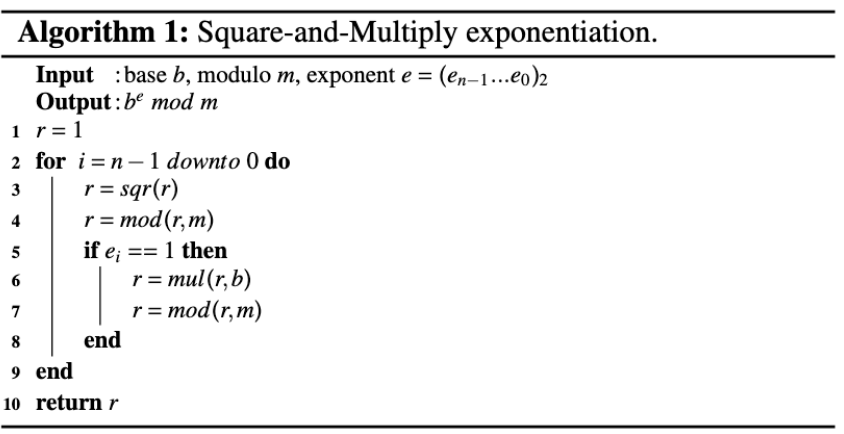
\includegraphics[scale=0.9]{../presentation/sqm.png}
\caption{Square and Multiply algorithm. Image from the SHARP paper~\cite{sharp}.}
\label{fig:sm}
\end{figure}

As an example, take the square and multiply algorithm~\cite{exp} used to compute encrypted messages for RSA encryption.
The program executing the algorithm in Figure~\ref{fig:sm}, which we call the {\it victim}, will execute line $6$ only when the current bit of the private exponent is 1. 
Regardless of the bit value, the victim will execute line $3$ after each iteration.
Note that the time between iterations is large because the instructions are often operating on big numbers ($> 2000$ bits).
If a malignant process, which we will call the {\it spy}, knows the victim's execution pattern of the lines $3$ and $6$, it can recover the encryption key used by the victim.

Many styles of cache side-channel attacks to recover the encryption key have been researched, including {\it flush and reload}, {\it evict and reload} and {\it prime and probe}, to name a few. 
We will focus on prime and probe attacks, which we exemplify in Figure~\ref{fig:pp}.
This attack assumes the victim and spy are running on different cores but share an L3 cache.
In addition, the spy must know which cache set the address of $mul$ (called in instruction $6$ in Figure~\ref{fig:sm}) is mapped to.
The attack begins with the spy priming the cache set through several load instructions.
In step $1$ the spy makes four loads to fill up the cache set with an associativity of four.
Then the victim may execute instruction $6$ and call the $mul$ function, loading it (represented as the green dot) into memory if there is an exponent in the encryption key.
During step $2$ the spy waits.
At step $3$ the spy reloads all four memory addresses, and if there is a miss the spy assumes the victim had an exponent bit.
Alternatively, if the victim did not have an exponent bit the spy should have all hits.
Ideally, the spy could run this attack on multiple uses of the victim's encryption key and combine the information found at each iteration.
This is important because the process is inherently noisy and other cores may be accessing memory in the same L3 cache set.
However, there are ways to extract a full encryption key from a partial key~\cite{partKey}.

A real-world implementation of this attack requires several pieces of information that can be found through experimentation.
The address of the desired instruction in memory and the wait time of the spy in step $2$ can be determined emperically~\cite{waitTime}.
Additionally, an L3 cache miss can be inferred by finding average L1, L2, and L3 miss times,
assuming there is a significant and measurable difference between L3 misses and the rest of the cache.
We do not focus on these platform specific numbers, and instead model our attacks at a high-level with these assumptions baked in.

\begin{figure}[t]
\centering
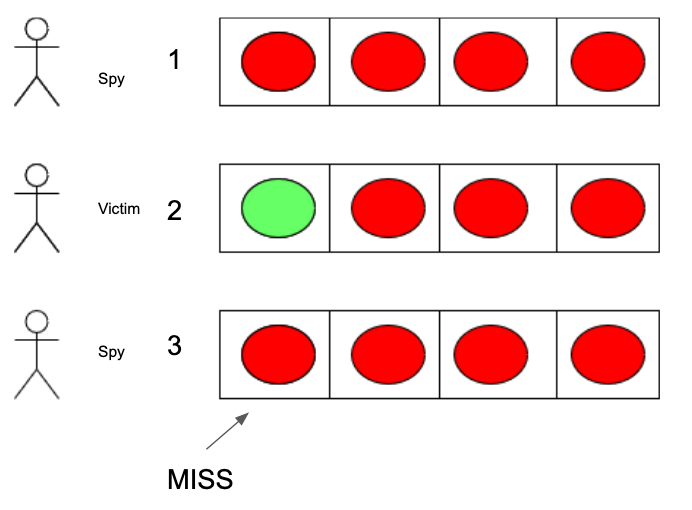
\includegraphics[scale=0.8]{../presentation/cattack.png}
\caption{Prime and probe attack showing content of a set in a 4-way L3 shared cache.}
\label{fig:pp}
\end{figure}

The {\it SHARP}~\cite{sharp} protocol presents one way of mitigating cache side-channel attacks by modifying the eviction policy for the shared L3.
Our project involved implementing high-level simulations of the SHARP protocol, 
then deploying two styles of prime and probe attacks that bypassed the protocol.
One attack uses multiple spies on multiple cores ({\it Multiple Spies}) and the other uses spies sharing the victims core ({\it Shared Core}).
We ran experiments on a deterministic python simulator as a proof of concept.
We then constructed a pintool to show that our attacks work even when some noise is added to the experiment.


\section{SHARP}

The Secure Hierarchy-Aware cache Replacement Policy (SHARP) is a cache eviction policy designed to work in a shared L3 cache and mitigate cache side-chanel attacks~\cite{sharp}.
The general idea of SHARP is to prevent {\it inclusion victims}.
An inclusion victim is created when data evicted in the shared L3 is active in a core's private L2 cache.
That data must then be evicted from the private L2 to preserve inclusivity.
Preventing inclusion victims should mitigate attacks of the sort in Figure~\ref{fig:pp} because the attack relies on the prime step which evicts the victims instruction from memory.
This would cause an inclusion victim and is therefore prevented.
So, when the spy tries to prime its four pieces of data into the shared L3,
it will not be able to fill the cache set and evict the victim.

It is infeasible to prevent inclusion victims in every case, e.g., a cache set may contain cache lines that all create inclusion victims if evicted leading to a deadlock scenario.
Therefore, the SHARP design provides a multi-step process for implementing the eviction policy when a core accesses memory:

\begin{enumerate}

\item If the cache set contains an unused cache line use it. Otherwise go to $2$.
\item If the cache set contains a cache line owned by the calling core, evict the cache line owned by the calling core based on the existing replacement policy ordering. Otherwise go to $3$.
\item Evict some cache line at random and increment the alarm counter for the calling core.

\end{enumerate}

The alarm counter helps identify when a core is causing frequent random evictions in step $3$.
This information can be used by the operating system to investigate processes running on a certain core. The authors recommend using a threshold of 2000 alarm triggers per core every one billion cycles to detect attacks. Legitimate executions should not surpass that value.
Core Valid Bits (CVBs) are used to determine when a cache line is owned by a core, i.e., the data is active in the core's private L2 cache.
SHARP describes three methods for maintaining the CVBs, involving lazy updates or snoopy monitoring.
In our implementation, we assume the CVBs are accurate under a snoopy protocol, meaning the CVB is set iff the data is active in the core's L2 cache. 
This is an important assumption for the shared core attack.

Since the SHARP paper was published in 2017, there has been research into problems with the protocol~\cite{howSharp}.
This work shows how the replacement policy can be exploited with denial of service attacks.
The attacker owns many cache lines and constantly forces the victim into the step $3$ random eviction.
It also investigates how useful the alarm counter is in detecting spies, and how the coarse-grained alarm counter lacks information on the thread level.
The paper also described a prime and probe attack to bypass SHARP, but the details are insufficient for replication.

We propose two attacks that bypass SHARP.
The first attack uses multiple spies each accessing a single cache line in the shared L3.
This takes advantage of the random eviction in step $3$ of the protocol.
The second attack uses a spy on the same core of the victim to invalidate the victim's data in the private L2 cache.
This takes advantage of the snoopy CVB monitoring, allowing a second spy to complete the basic prime and probe attack.

\section{Multiple Spy Attack}

\begin{figure}[h]
\centering
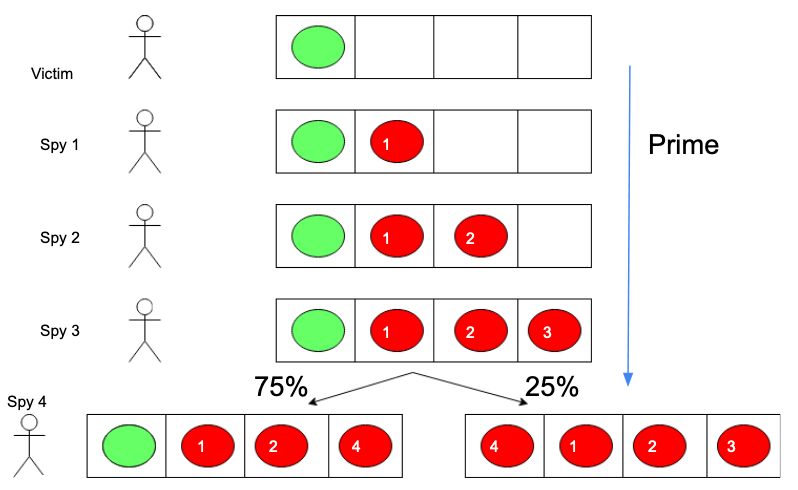
\includegraphics[scale=0.9]{../presentation/shared.png}
\caption{Example of a multiple spy attack at the level three shared cache with a set size of four.}
\label{fig:ms}
\end{figure}

The multiple spy attack takes advantage of the random eviction in step $3$ of SHARP by placing spies on $n$ cores assuming the associativity of the L3 cache is $n$.
Figure~\ref{fig:ms} shows the basic setup for the attack.
Assuming the victim has active data in the L3, $n-1$ spies will load independent data into a single cache line.
Then the $n^{th}$ spy loads data with a $\frac{1}{n}$ chance of evicting the victim (shown by the $25\%$ case in the example).
The spies then wait for some time and all reload their data, recording any misses at the L3 cache.
It is important that the $n^{th}$ spy reload its data first, as this allows more information to be gained.
The exponent bit can be inferred in the following cases for each iteration:

\begin{enumerate}

\item The exponent bit is $0$ if all spies have cache hits. This means the victim never put data into the cache set.
\item The exponent bit is $1$ if all spies had cache hits in the previous iteration and some spies have cache misses in the current iteration. This means the victim may have put data into the cache set causing a cache miss.
\item The exponent bit is $1$ if the $n^{th}$ spy which loads first after the victim has a cache miss. The $n^{th}$ spy was the last to load during the prime stage, so no other spy could have evicted its data. This means the victim may have evicted it. This happens with probability $\frac{1}{n}$ as the victim would evict some spy at random.
\item Otherwise, the exponent bit is unknown (we represent this a $-1$ in our simulations).

\end{enumerate}

Of course, for case $2$ and $3$ it may be another program that puts data into the cache set.
Additionally, the chances that you can learn information are slightly better than $\frac{1}{n}$ (due to the order of spy loads).
So, there will be many $-1$'s in the recovered key, and potentially some $1$'s that are incorrectly labelled. 
We account for this by running the attack over many victim's executions.
Then the set of partial keys are combined.
Since the eviction is random, the chances of at least one of the spies' primes working (right-hand side of Figure~\ref{fig:ms}) for a specific bit in the key become more likely with each additional execution.
As an aside, case $3$ requires timing between the loads of the $n^{th}$ spy and the other spies, which may be unrealistic for spies acting across several cores.

In this attack, the alarm counter for both the victim and the $n^{th}$ spy would be incremented during the random evictions.
However, the alarms can be spread across all spies by rotating which spy makes the $n^{th}$ load.
This rotation can be based on a predefined static schedule, so the spies would not need to communicate.


\section{Shared Core Attack}

\begin{figure}[h]
\centering
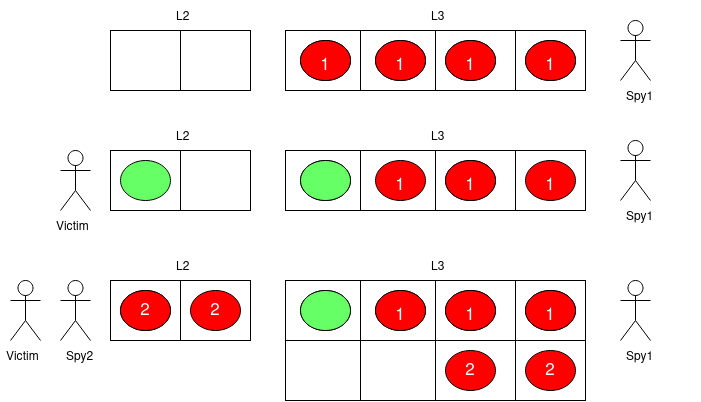
\includegraphics[scale=0.5]{../presentation/snd_atk.png}
\caption{Example of a shared core attack at the level two private and 4-way level three shared cache.}
\label{fig:ss}
\end{figure}

The shared core attack relies on the assumption that the CVBs operate using a snoopy protocol.
This allows a spy on the same core as the victim to invalidate memory at the private L2.
Figure~\ref{fig:ss} shows an example of this attack, where the L2 is a private cache shared between Spy2 and the victim.
In this attack Spy1 is tasked with priming the shared L3 cache set and collecting information about the encryption key exponents.
To do this, Spy1 first primes the cache set with $n$ loads.
Then Spy1 waits as the victim accesses the exponent bit instruction, bringing that instruction into the L3 and L2.
After the victim has accessed the instruction, Spy2 fills the L2 set containing the victim's data.
If the L2 uses an LRU-based protocol, this will evict the victim's data.
Note that this data should be mapped to a separate cache set in the shared L3.
It is crucial that at this point the snoopy monitoring invalidates the CVB for the victim's data in the L3.
Finally, Spy1 reloads $n$ times encountering one miss if the victim has accessed data.
This miss allows the spy to infer a bit of value $1$, and all hits corresponds to value $0$.
Importantly, on the miss Spy1 will evict the now inactive victim cache line and once again fill the entire cache set.
This would not be possible if the victim data was still in the private L2.

This attack benefits from avoiding step $3$ in the SHARP protocol, so no random evictions will occur for the spies.
In addition, Spy1 will never increment its alarm counter because it never loads more than $n$ independent cache lines.
On the other hand, the victim will increase its alarm counter with each access to the exponent instruction.
This inverts the intended affect of the alarm counter.
For this attack it may be difficult to consistently evict data in the L2 with Spy2.
Since the processes share the same core it is not clear how thread scheduling and blocking on a cache miss would affect Spy2.

\section{Evaluation}

We implemented two simulators to model our attacks.
The first was a high-level simulator built in Python.
This simulator implements the SHARP protocol and both attacks, along with a representation of the L2 and L3 cache lines in question.
It abstracts away instructions and timing, meaning the encryption key either has an exponent bit and the victim accesses memory or it does not.
The square and multiply algorithm is not implemented.
The spies are also assumed to know the appropriate wait time and recognize cache misses correctly.

This was simply a prototype to quickly evaluate the two attacks under near perfect conditions.
The tool can be used with the following options:

\begin{itemize}
\item -s  Cache set size (spawn same number of spies for multiple spies attack)
\item -k  RSA key exponents, e.g. 011000110
\item -i  Iterations of RSA key detection
\item -a 1 for multiple spies attack, 2 for shared core attack
\end{itemize}

We sought to further evaluate the attacks in a more robust simulation framework that included noise.
To do this we decided to use a pintool.
This was the best option, as the simulators used in~\cite{sharp,howSharp} had poor documentation and the authors of SHARP were unable to give us their source code.
Pintool does not have support for inserting analysis code into multiple executable files that are running on multiple cores simultaneously. 
To get around this, we used the victim program~\footnote{RSA implementation found at \\\url{https://gist.github.com/Thelouras58/a3b04a3df0d167743084ff94442f52d8}} as the executable.
The spies, cache hierarchy, SHARP protocol, and global timing were implemented in the pintool itself.

Describe Implementation 

Describe Resulsts

\section{Conclusion and Future Work}

In this work we implemented the SHARP protocol for a high-level deterministic simulator and also as a pintool.
We implemented two cache side-channel attacks that recover the bits of an encryption key for the RSA algorithm.
The experimentation shows a proof-of-concept for the attacks, with some level of noise added to the pintool.
To make the attacks more enticing, it would be important to implement them on a multi-core cycle-level simulator.
This would add more noise to the system and bring the attacks closer to real-world implementation.
This requires significant additional work, including empirically determining spy wait times, instruction addresses in the shared L3, and L2/L3 approximate miss times.

In the project proposal $75\%$ was to implement SHARP in a simulated environment and evaluate the protocol, $100\%$ was to design attacks to bypass SHARP, and $125\%$ involved evaluating more mitigation techniques beyond SHARP. 
We feel we landed comfortably in the $100\%$ range.
We were very happy with the two attacks we came up with, and decided to spend more time on them than implementing SHARP in a more sophisticated simulator.
The largest setback was realizing the simulators used in the relevant papers~\cite{sharp,howSharp} had little developer support.
We reached out to the author of SHARP but they were not able to share the source code they used for experimentation.
As such, we opted for a solution that hacked spies into pintool.
It added some noise, taking the experimentation a level above the deterministic simulator we implemented in Python.

Source code can be found at\\ \url{https://github.com/icemonster/mitigatingCacheSideChannels}.


\newpage

\bibliographystyle{plain}
\bibliography{cattack}

\end{document}
